\documentclass[15pt]{article}
\usepackage[utf8]{inputenc}
\pagestyle{plain}
\usepackage[
top    = 2.75cm,
bottom = 2.55cm,
left   = 3.00cm,
right  = 3.00cm]{geometry}
\usepackage{graphicx,amsmath}
\usepackage{xcolor}

\pagecolor[RGB]{18,18,18} %blackish
\color[rgb]{0.9, 0.9, 0.9} %greyish

\usepackage{hyperref}
\usepackage{titlesec}
\usepackage{tocloft}
\usepackage[none]{tocbibind}
\usepackage{float}
\usepackage{fancyhdr}

\titleformat*{\subsection}{\normalfont}
\graphicspath{ {./HS101 images/} }
\definecolor{- }{RGB}{80,203,147}
\definecolor{green}{RGB}{113,239,163}
\setcounter{secnumdepth}{5}
\setcounter{tocdepth}{1}

\pagestyle{fancy}
\fancyhf{}
\renewcommand{\headrulewidth}{0pt}
\renewcommand{\footrulewidth}{0.4pt}
\fancyfoot[R]{ADI}
\fancyfoot[L]{\thepage}

\renewcommand{\b}[1]{\begin{#1}}
\newcommand{\e}[1]{\end{#1}}
\renewcommand{\i}{\item{}}
\newcommand{\tb}[1]{\textbf{#1}}
\renewcommand{\thefigure}{}
\renewcommand{\cfttoctitlefont}{\Huge}

\b{document}
   \b{center}
       \vspace*{12cm}
       \tb{{\Huge HS101 Short Notes}}
       
       \vspace{0.9cm}
       \tb{\LARGE Aditya Byju}
            
       \vspace{0.5cm}
       \large {\tb{Course Professor:} Prof. Krishnan Narayanan\\
       \tb{Ref:} Prof's slides, Principles of Microeconomics by N. Gregory Mankiw\\
       Know that, economics is a very dangerous science\hspace{0.05cm}!}
       
       \vspace{0.5cm}
       \tb{Economics}
       
       \vspace{0.5cm}
       September 2021
            
       \vspace{0.8cm}
    \e{center}
\thispagestyle{empty}

\newpage
\tableofcontents
\addtocontents{toc}{\vspace{0.2cm}}

\newpage
\phantomsection
\section*{\color{- }Introduction}
\addcontentsline{toc}{section}{\large\color{- }Introduction}

\b{itemize}
    \i \tb{economy} - comes from Greek word {\color{green}oikonomos} - means ``one who manages a household"
    \i \tb{scarcity} - the limited nature of society's resources
    \i \tb{economics} - the study of how society manages its scarce resources
\e{itemize}

\phantomsection
\section*{\color{- }Ten principles of Economics}
\addcontentsline{toc}{section}{\large\color{- }Ten principles of Economics}
\subsection*{How people make decisions:}
\b{enumerate}
    \i \tb{People face Trade-offs}
    \b{itemize}
        \i \tb{efficiency} - society getting the most it can from its scarce resources
        \i \tb{equality} - distributing economic prosperity uniformly among the members of society
        \i \tb{equity} - means the benefits of those resources are distributed fairly among the members of society
    \e{itemize}
    \i \tb{The cost of something is what you give up to get it}
    \b{itemize}
        \i \tb{opportunity cost} - whatever must be given up to obtain some item
    \e{itemize}
    \i \tb{Rational people think at the margin}
    \b{itemize}
        \i \tb{rational people} - people who systematically and purposefully do the best they can to achieve their objectives
        \i \tb{marginal changes} - small incremental adjustments to a plan of action
        \i Rational people often make decisions by comparing marginal benefits and marginal costs
        \i A person's willingness to pay for any good is based on the marginal benefit that an extra unit of the good would yield (e.g. think of cost and utilization of water vs. diamond)
    \e{itemize}
    \i \tb{People respond to incentives}
    \b{itemize}
        \i \tb{incentive} - something that induces a person to act
        \i When analyzing any policy, we must consider not only the direct effects but also the less obvious indirect effects that work through incentives. If the policy changes incentives, it will cause people to alter their behaviour. 
    \e{itemize}
\e{enumerate}

\subsection*{How people interact:}
\b{enumerate}
\setcounter{enumi}{4}
    \i \tb{Trade can make everyone better off}
    \b{itemize}
        \i Trade allows each person to specialize in the activities he or she does best. By trading with others people can buy a greater variety of goods and services at lower cost.
    \e{itemize}
    \i \tb{Markets are usually a good way to organize economic activity}
    \b{itemize}
        \i \tb{market economy} - an economy that allocates resources through the decentralized decisions of many firms as they interact in markets for goods and services
        \i Adam Smith in his book \emph{An Inquiry into the Nature and Causes of the Wealth of Nations} said households and firms interacting in markets act as if they are guided by an {\color{green}`invisible hand'} that leads them to desirable market outcomes
        \i Prices are the instrument with which the invisible hand directs economic activity. Prices adjust to guide the individual buyers and sellers to reach outcomes that, in many cases, maximize the well-being of a society as a whole.
    \e{itemize}
    \i \tb{Governments can sometimes improve market outcomes}
    \begin{itemize}
        \i The invisible hand can work its magic only if the government enforces the rules and maintains the institutions that are key to a market economy. Market economies need institutions to enforce {\color{green}property rights} so individuals can own and control scarce resources.
        \i \tb{property rights} - the ability of an individual to own and exercise control over scarce resources
        \i There are two broad reasons for a government to intervene in the economy and change the allocation of resources that people would choose on their own: {\color{green}to promote efficiency or to promote equality}
        \i \tb{market failure} -  a situation in which a market left on its own fails to allocate resources efficiently
        \i \tb{externality} - the impact of one person's actions on the well-being of a bystander
        \i \tb{market power} - the ability of a single economic actor (or small group of actors) to have a substantial influence on market prices
    \end{itemize}
\e{enumerate}
 
\subsection*{How the economy as a whole works:}
\b{enumerate}
\setcounter{enumi}{7}
    \i \tb{A country's standard of living depends on its ability to produce goods and services}
    \b{itemize}
        \i Almost all variation in living standards is attributable to differences in countries' {\color{green}productivity}
        \i \tb{productivity} - the quantity of goods and services produced from each unit of labor input
        \i The growth rate of a nation's productivity determines the growth rate of its average income
    \e{itemize}
    \i \tb{Prices rise when the government prints too much money}
    \b{itemize}
        \i \tb{inflation} - an increase in the overall level of prices in the economy
        \i In almost all cases of large or persistent inflation, the culprit is growth in the quantity of money
    \e{itemize}
    \i \tb{Society faces a short-run trade-off between inflation and unemployment}
    \b{itemize}
        \i Most economists describe the short-run effects of monetary injections as follows:
        \b{itemize}
            \item[$-$] Increasing the amount of money in the economy stimulates the overall level of spending and thus the demand for goods and services.
            \item[$-$] Higher demand may over time cause firms to raise their prices, but in the meantime, it also encourages them to hire more workers and produce a larger quantity of goods and services.
            \item[$-$] More hiring means lower unemployment.
        \e{itemize}
        \i \tb{business cycle} - fluctuations in economic activity, such as employment and production
    \e{itemize}
\e{enumerate}

\phantomsection
\section*{\color{- }Economic Models}
\addcontentsline{toc}{section}{\large\color{- }Economic Models}
\b{itemize}
    \i Economists use models which are most often composed of diagrams and equations to learn about the world 
\e{itemize}
\subsection*{\tb{First model: The Circular-flow Diagram}}
\b{itemize}
    \i \tb{circular-flow diagram} - a visual model of the economy that shows how money flows through markets among households and firms
\e{itemize}
\begin{figure}[H]
\centering
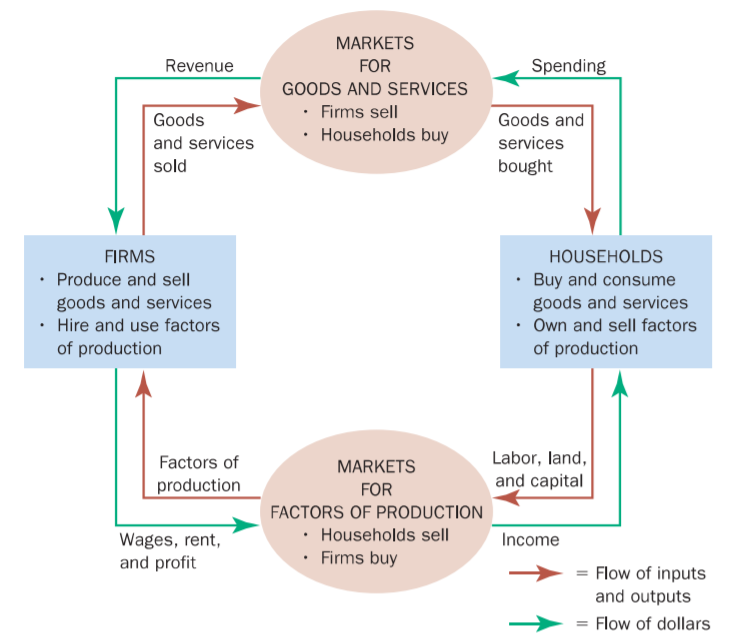
\includegraphics[width=11cm]{HS101 images/The Circular-flow Diagram.png}
\end{figure}
\b{itemize}
    \i In this model, the economy is simplifies to include only two types of decision makers - firms and households. Firms produce goods and services using inputs, such as labor, land, and capital (buildings and machines). These inputs are called the {\color{green}factors of production}. households own  the factors of production and consume all the goods and services that the firms produce.
    \i The two loops of the circular-flow diagram are distinct but related. The inner loop represents the flow of inputs and outputs. The outer loop represents the corresponding flow of money.
    \i This is a basic circular-flow model,  a more complex and realistic one would include, for instance, the roles of government and international trade
\e{itemize}
\subsection*{\tb{Second model: The Production Possibilities Frontier}}
\b{itemize}
    \i \tb{production possibilities frontier} - a graph that shows the combinations of output that the economy can possibly produce given the available factors of production and the available production technology
\e{itemize}
\begin{figure}[H]
\centering
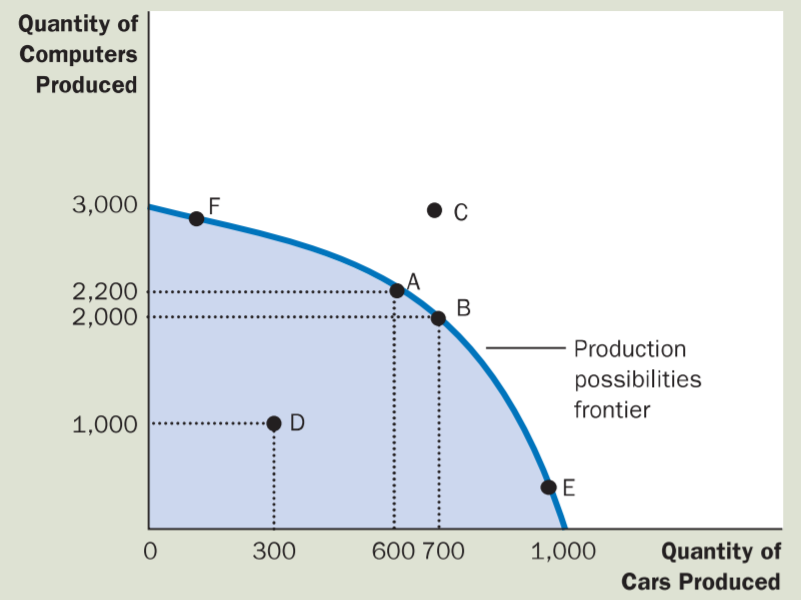
\includegraphics[width=11cm]{HS101 images/The Production Possibilities Frontier.png}
\caption{Production Possibilities Frontier in an example of cars and computers}
\end{figure}
\b{itemize}
    \i With the resources it has, the economy can produce at any point on or inside the production possibilities frontier, but it cannot produce at points outside the frontier
    \i An outcome is said to be {\color{green}efficient} if the economy is getting all it can from the scarce resources it has available. Points on (rather than inside) the production possibilities frontier represent efficient levels of production.
    \i Here the opportunity cost of a car can be represented as the slope of the Production Possibilities Frontier
\e{itemize}

\phantomsection
\section*{\color{- }Microeconomics and Macroeconomics}
\addcontentsline{toc}{section}{\large\color{- }Microeconomics and Macroeconomics}
\b{itemize}
    \i \tb{microeconomics} - the study of how house-holds and firms make decisions and how they interact in markets
    \i \tb{macroeconomics} - the study of economy-wide phenomena, including inflation, unemployment, and economic growth
    \i Microeconomics and macroeconomics are closely intertwined as changes in the overall economy arise from the decisions of millions of individuals
\e{itemize}

\phantomsection
\section*{\color{- }The economist as scientist/policy adviser}
\addcontentsline{toc}{section}{\large\color{- }The economist as scientist/policy adviser}
\subsection*{\tb{The economist as scientist}}
\b{itemize}
    \i Economists try to address their subject with a scientist's objectivity. They approach the study of the economy in much the same way a physicist approaches the study of matter and a biologist approaches the study of life: They devise theories, collect data, and then analyze these data in an attempt to verify or refute their theories.
\e{itemize}
\subsection*{\tb{The economist as policy adviser}}
\b{itemize}
    \i Economists act as policy advisers when they are asked to recommend policies to improve economic outcomes
    \i \tb{positive statements} - claims that attempt to describe the world as it is. Positive statements are {\color{green}descriptive.}
    \i \tb{normative statements} - claims that attempt to prescribe how the world should be. Normative statements are {\color{green}prescriptive.}
\e{itemize}
 
\phantomsection
\section*{\color{- }Why economists disagree?}
\addcontentsline{toc}{section}{\large\color{- }Why economists disagree?}
There are two basic reasons:
\b{itemize}
    \i Economists may disagree about the validity of alternative positive theories about how the world works
    \i Economists may have different values and therefore different normative views about what policy should try to accomplish
\e{itemize}

\phantomsection
\section*{\color{- }Comparative advantage : The driving force of specialization}
\addcontentsline{toc}{section}{\large\color{- }Comparative advantage : The driving force of specialization}
\b{itemize}
    \i \tb{absolute advantage} - the ability to produce a good using fewer inputs than another producer
    \i \tb{comparative advantage} - the ability to produce a good a t a lower opportunity cost than another producer
    \i Considering a case of trade between two people (and two goods), although it is possible to have an absolute advantage in both goods, it is impossible for one person to have a comparative advantage in both goods. Unless two people have exactly the same opportunity cost, one person will have a comparative advantage in one good, and the other person will have a comparative advantage in the other good.
    \i The gains from specialization and trade are based not on absolute advantage but on comparative advantage. When each person specializes in producing the good for which he or she has a comparative advantage, total production in the economy rises. This increase in the size of the economic pie can be used to make everyone better off.
    \i The price of the trade:
    \b{itemize}
        \item[$-$] For both parties to gain from trade, the price at which they trade must lie between the two opportunity costs
    \e{itemize}
\e{itemize}

\phantomsection
\section*{\color{- }The market forces of supply and demand}
\addcontentsline{toc}{section}{\large\color{- }The market forces of supply and demand}
\b{itemize}
    \i \tb{market} - a group of buyers and sellers of a particular good or service
    \i \tb{competitive market} - a market in which there are many buyers and many sellers so that each has a negligible impact on the market price
    \i \tb{monopoly} - some markets have only one seller, and this seller sets the price. Such a seller is called a monopoly.
\e{itemize}

\phantomsection
\section*{\color{- }Demand and the demand curve}
\addcontentsline{toc}{section}{\large\color{- }Demand and the demand curve}
\b{itemize}
    \i \tb{quantity demanded} - the amount of a good that buyers are willing and able to purchase
    \i \tb{law of demand} - the claim that, other things equal, the quantity demanded of a good falls when the price of the good rises
    \i \tb{demand schedule} - a table that shows the relationship between the price of a good and the quantity demanded
    \i \tb{demand curve} - a graph of the relationship between the price of a good and the quantity demanded
\e{itemize}
\begin{figure}[H]
\centering
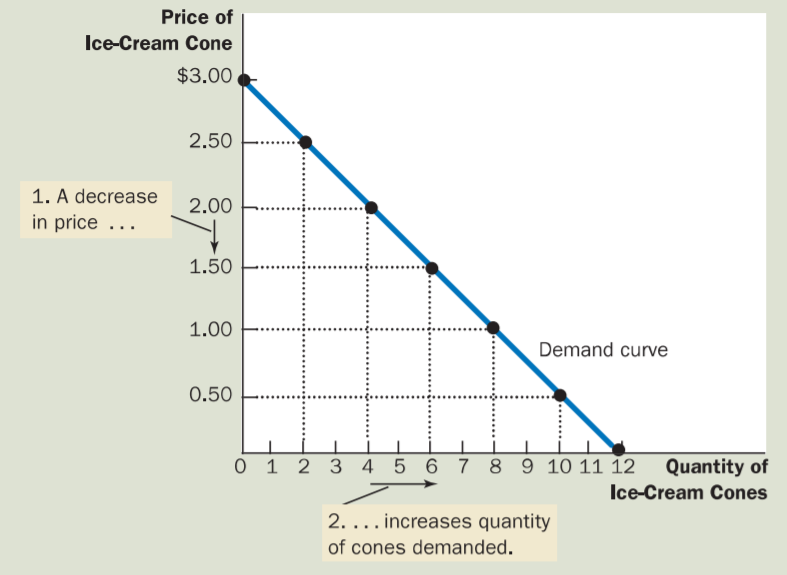
\includegraphics[width=11cm]{HS101 images/Demand curve for an example of ice-cream cones.png}
\caption{Demand curve for an example of ice-cream cones}
\end{figure}
\b{itemize}
    \i \tb{market demand} - the sum of all the individual demands for a particular good or service
    \i Shifts in the demand curve:
    \b{itemize}
        \item[$-$] Any change that raises the quantity that buyers wish to purchase at any given price shifts the demand curve to the right
        \item[$-$] Any change that lowers the quantity that buyers wish to purchase at any given price shifts the demand curve to the left
    \e{itemize}
    \begin{figure}[H]
    \centering
    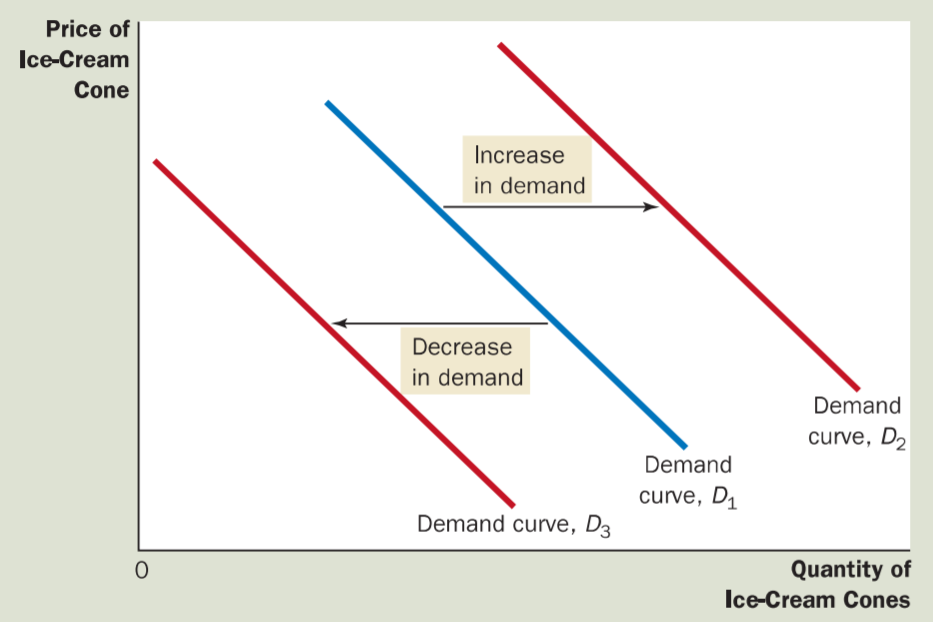
\includegraphics[width=11cm]{HS101 images/Shifts in the demand curve.png}
    \caption{Shifts in the Demand curve}
    \end{figure}
    \i \tb{normal good} - a good for which, other things equal, an increase in income leads to an increase in demand
    \i \tb{inferior good} - a good for which, other things equal, an increase in income leads to an decrease in demand
    \i \tb{substitutes} - two goods for which an increase in the price of one leads to an increase in the demand for the other. They are often pairs of goods that are used in place of each other.
    \i \tb{complements} - two goods for which an increase in the price of one leads to a decrease in the demand for the other. They are often pairs of goods that are used together.
    \i Remember that a curve shifts when there is a change in a relevant variable that is not measured on either axis. Because the price is on the vertical axis, a change in price represents a movement along the demand curve. By contrast, income, the prices of related goods,  tastes, expectations, and the number of buyers are not measured on either axis, so a change in one of these variables shifts the demand curve.
\e{itemize} 

\phantomsection
\section*{\color{- }Supply and the supply curve}
\addcontentsline{toc}{section}{\large\color{- }Supply and the supply curve}
\b{itemize}
    \i \tb{quantity supplied} - the amount of a good that sellers are willing and able to sell
    \i \tb{law of supply} - the claim that, other things equal, the quantity supplied of a good rises when the price of the good rises
    \i \tb{supply schedule} - a table that shows the relationship between the price of a good and the quantity supplied
    \i \tb{supply curve} - a graph of the relationship between the price of a good and the quantity supplied 
\e{itemize}
\begin{figure}[H]
\centering
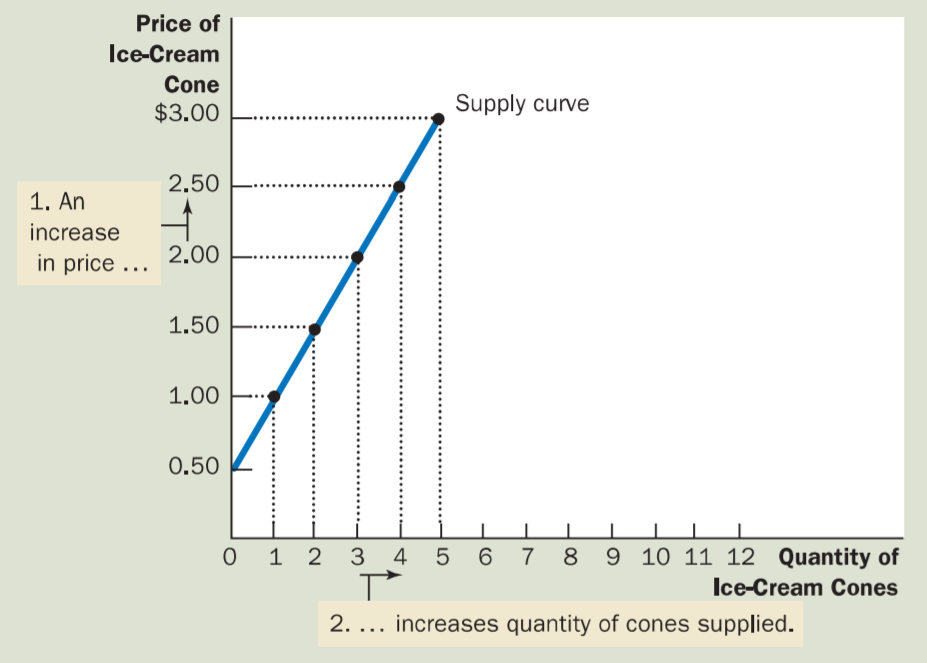
\includegraphics[width=9.5cm]{HS101 images/Supply curve for an example of ice-cream cones.png}
\caption{Supply curve for an example of ice-cream cones}
\end{figure}
\b{itemize}
    \i \tb{market supply} - the sum of all the individual supplies for a particular good or service
    \i Shifts in the supply curve:
    \b{itemize}
        \item[$-$] Any change that raises the quantity that sellers wish to produce at any given price shifts the supply curve to the right
        \item[$-$] Any change that lowers the quantity that sellers wish to produce at any given price shifts the supply curve to the left
    \e{itemize}
    \begin{figure}[H]
    \centering
    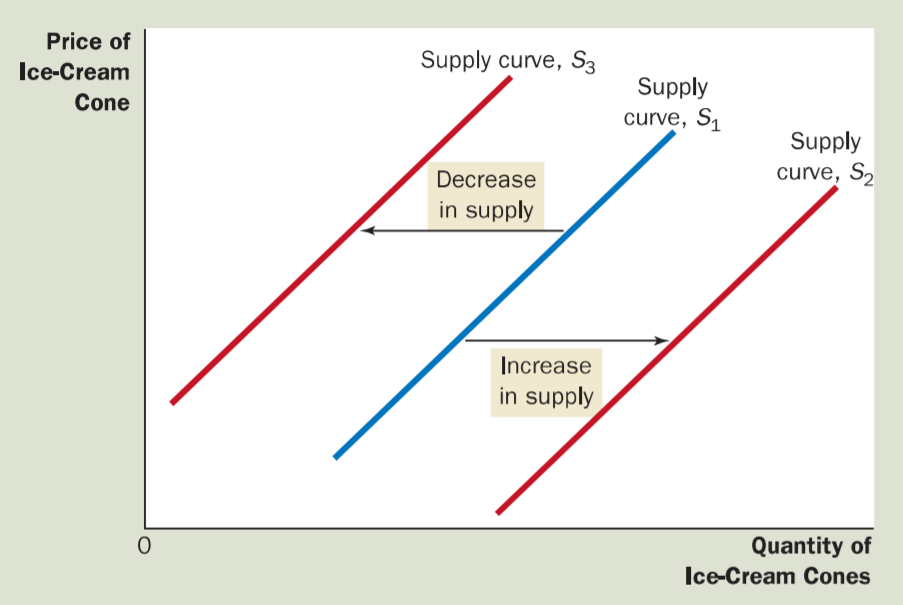
\includegraphics[width=9.5cm]{HS101 images/Shifts in the supply curve.png}
    \caption{Shifts in the Supply curve}
    \end{figure}
    \i Remember that a curve shifts when there is a change in a relevant variable that is not measured on either axis. Because the price is on the vertical axis, a change in price represents a movement along the supply curve. By contrast, because input prices, technology, expectations, and the number of sellers are not measured on either axis, so a change in one of these variables shifts the supply curve.
\e{itemize}

\phantomsection
\section*{\color{- }Supply and demand together}
\addcontentsline{toc}{section}{\large\color{- }Supply and demand together}
\b{itemize}
    \begin{figure}[H]
    \centering
    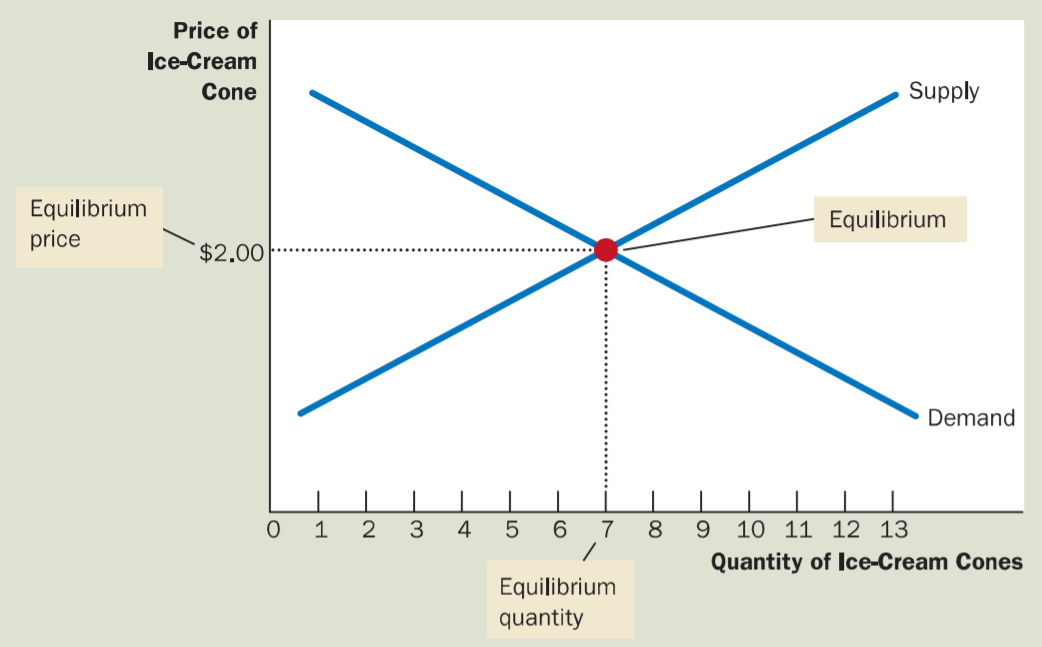
\includegraphics[width=11cm]{HS101 images/The equilibrium of supply and demand in case of ice-cream cones.png}
    \caption{The equilibrium of supply and demand in case of ice-cream cones}
    \end{figure}
    \i \tb{equilibrium} - a situation in which the market price has reached the level at which quantity supplied equals quantity demanded
    \i \tb{equilibrium price (market-clearing price)} - the price that balances quantity supplied and quantity demanded
    \i \tb{equilibrium quantity} - the quantity supplies and the quantity demanded at the equilibrium price
    \begin{figure}[H]
    \centering
    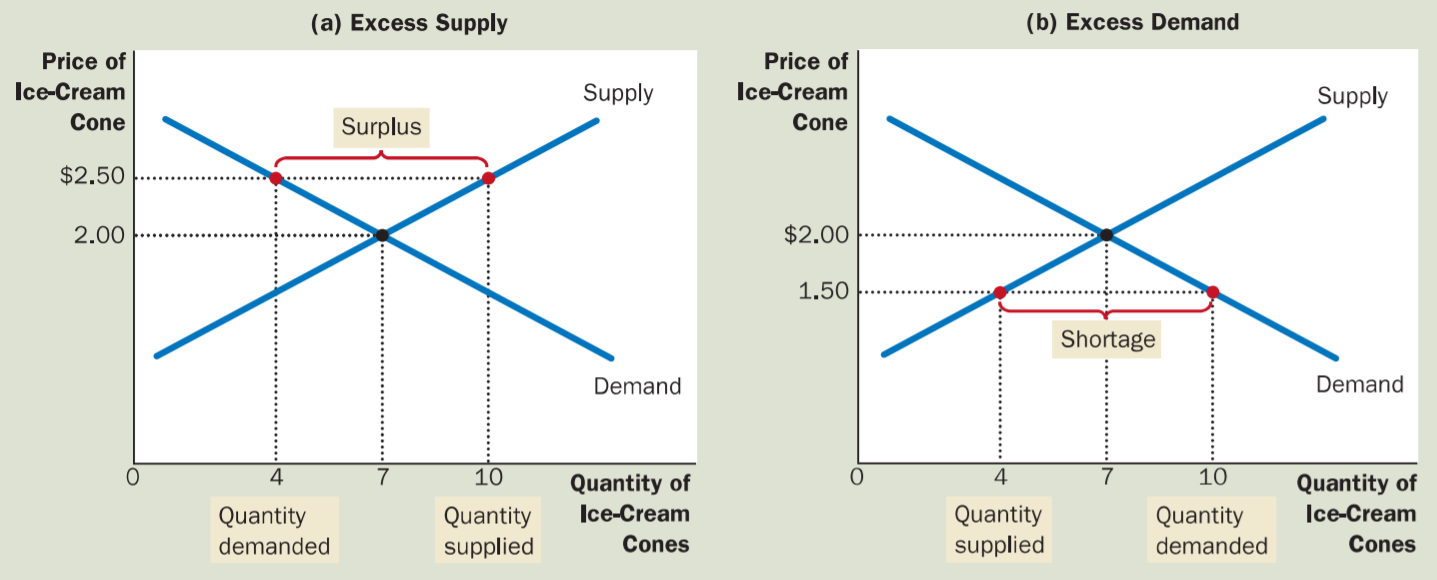
\includegraphics[width=11cm]{HS101 images/Markets not in equilibrium.png}
    \caption{Markets not in equilibrium}
    \end{figure}
    \i \tb{surplus} - a situation in which quantity supplied is greater than quantity demanded. It is also called a situation of excess supply. 
    \i \tb{shortage} - a situation in which quantity demanded is greater than quantity supplied. It is also called a situation of excess demand. 
    \i \tb{law of supply and demand} - the claim that the price of any good adjusts to bring the quantity supplied and the quantity demanded for that good into balance
    \i Three steps to analyzing changes in equilibrium:
    \b{itemize}
        \item[$-$] Decide whether the event shifts the supply or demand curve (or perhaps both) 
        \item[$-$] Decide in which direction the curve shifts
        \item[$-$] Use the supply-and-demand diagram to see how the shift changes the equilibrium price and quantity
    \e{itemize}
    \i A shift in the supply curve is called a {\color{green}change in supply}, and a shift in demand curve is called a {\color{green}change in demand}. A movement along a fixed supply curve is called a {\color{green}change in the quantity supplied}, and a movement along a fixed demand curve is called a {\color{green}change in the quantity demanded.}
    \begin{figure}[H]
    \centering
    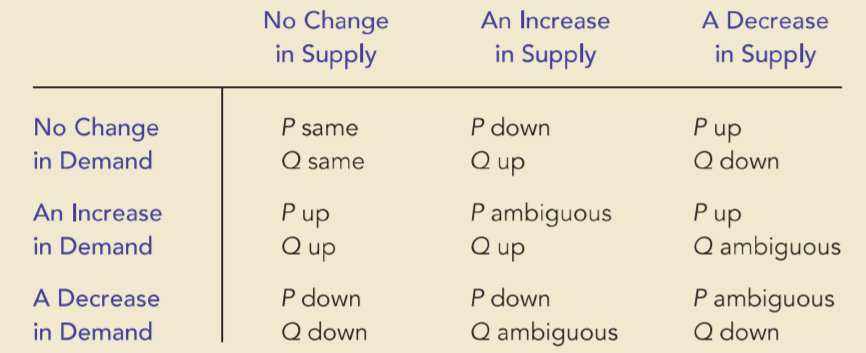
\includegraphics[width=11cm]{HS101 images/What happens to Price and Quantity when supply or demand shifts.png}
    \caption{What happens to Price and Quantity when supply or demand shifts? (P $\rightarrow$ Price, Q $\rightarrow$ Quantity)}
    \end{figure}
\e{itemize} 

\phantomsection
\section*{\color{- }Elasticity and its applications}
\addcontentsline{toc}{section}{\large\color{- }Elasticity and its applications}
\b{itemize}
    \i \tb{elasticity} - a measure of the responsiveness of quantity demanded or quantity supplied to one of its determinants
    \i Demand/Supply for a good is said to be elastic if the quantity demanded/supplied responds substantially to changes in the price. Demand/Supply for a good is said to be inelastic if the quantity demanded/supplied responds only slightly to changes in the price.
    \i \tb{price elasticity of demand} - a measure of how much the quantity demanded of a good responds to a change in the price of that good, computed as the percentage change in quantity demanded divided by the percentage change in price
    \begin{figure}[H]
    \centering
    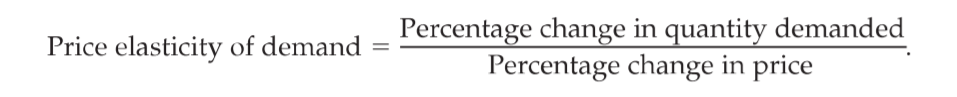
\includegraphics[width=11cm]{HS101 images/Price elasticity of demand equation.png}
    \end{figure}
    \i Midpoint method for calculating price elasticity of demand:
    \begin{figure}[H]
    \centering
    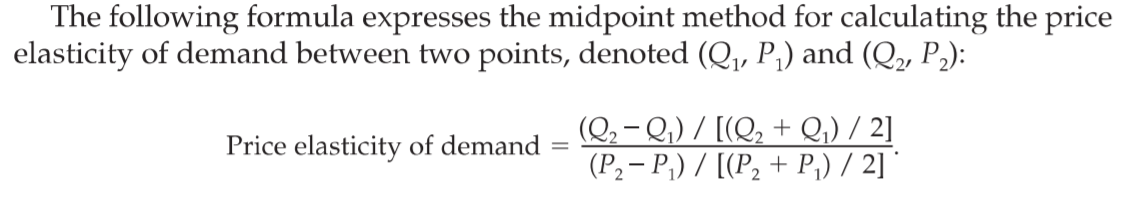
\includegraphics[width=11cm]{HS101 images/Midpoint method (price elasticity of demand).png}
    \end{figure}
    \i We normally take absolute value of price elasticity of demand
    \i Goods with close substitutes tend to have more elastic demand because it is easier for consumers to switch from that good to others. Necessities tend to have inelastic demands, whereas luxuries have elastic demands.
    \i Narrowly defined markets tend to have more elastic demand than broadly defined markets because it is easier to find close substitutes for narrowly defined goods
    \i Goods tend to have more elastic demand over longer time horizons
    \i Demand is considered {\color{green}elastic} when the elasticity is greater than 1, which means the quantity moves proportionately more than the price. Demand is considered {\color{green}inelastic} when the elasticity is less than 1, which means the quantity moves proportionately less than the price. If the elasticity is exactly equal to 1, the quantity moves the same amount proportionately as the price, and demand is said to have {\color{green}unit elasticity.}
    \begin{figure}[H]
    \centering
    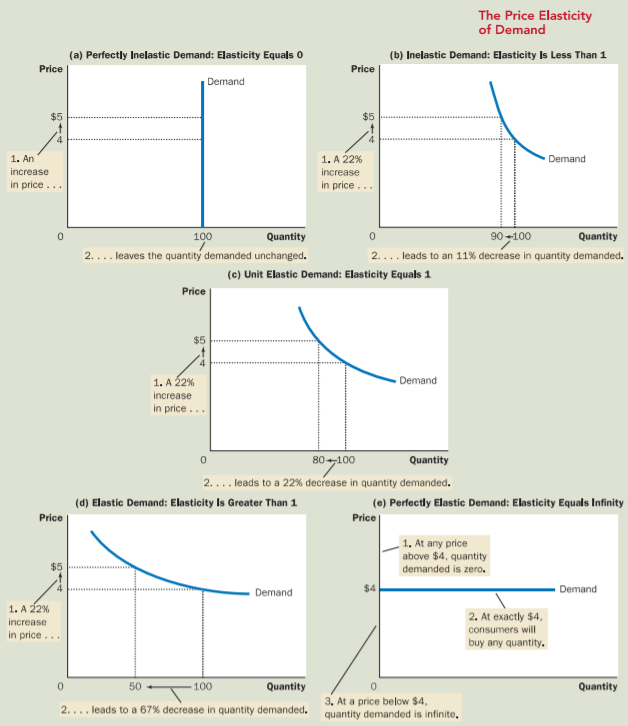
\includegraphics[width=14cm]{HS101 images/Diff. elasticity demand curves.png}
    \end{figure}
    \i The flatter the demand curve passes through a given point, the greater the price elasticity of demand. The steeper the demand curve that passes through a given point, the smaller the price elasticity of demand.
    \i \tb{total revenue} - the amount paid by buyers and sellers of a good, computed as the price of the good times the quantity sold
    \i Some general rules:
    \b{itemize}
        \item[$-$] When demand is inelastic, price and total revenue move in the same direction
        \item[$-$] When demand is elastic, price and total revenue move in opposite directions
        \item[$-$] If demand is unit elastic, total revenue remains constant when the price changes
    \e{itemize}
    \i \tb{income elasticity of demand} - a measure of how much the quantity demanded of a good responds to a change in consumer's income, computed as the percentage change in quantity demanded divided by the percentage change in income\\
    \begin{figure}[H]
    \centering
    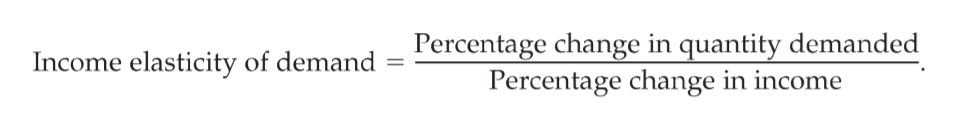
\includegraphics[width=11cm]{HS101 images/Income elasticity of demand equation.png}
    \end{figure} 
    \i \tb{cross-price elasticity of demand} - a measure of how much the quantity demanded of one good responds to a change in the price of another good, computed as the percentage change in quantity demanded of the first good divided by the percentage change in the price of the second good\\
    \begin{figure}[H]
    \centering
    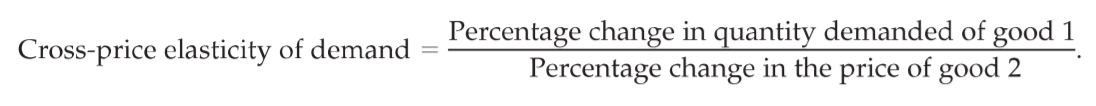
\includegraphics[width=11cm]{HS101 images/Cross-price elasticity of demand equation.png}
    \end{figure} 
    \i \tb{price elasticity of supply} - a measure of how much the quantity supplied of a good responds to a change in the price of that good, computed as the percentage change in quantity supplied divided by the percentage change in price\\
    \begin{figure}[H]
    \centering
    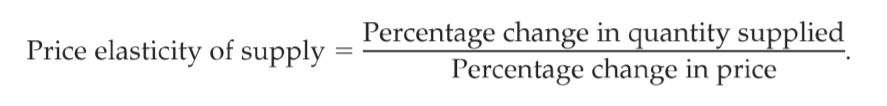
\includegraphics[width=11cm]{HS101 images/Price elasticity of supply equation.png}
    \end{figure}
    \i The price elasticity of supply measures the responsiveness of quantity supplied to the price, hence it is reflected in the appearance of the supply curve
    \i In the extreme case of a zero elasticity, the supply is perfectly inelastic, and the supply curve is vertical. In this case, the quantity supplied is the same regardless of the price. As the elasticity rises, the supply curve gets flatter, which shows that the quantity supplied responds more to changes in the price. Supply is perfectly elastic when the price elasticity of supply approaches infinity and the supply curve becomes horizontal, meaning that very small changes in the price lead to very large changes in the quantity supplied.
    \begin{figure}[H]
    \centering
    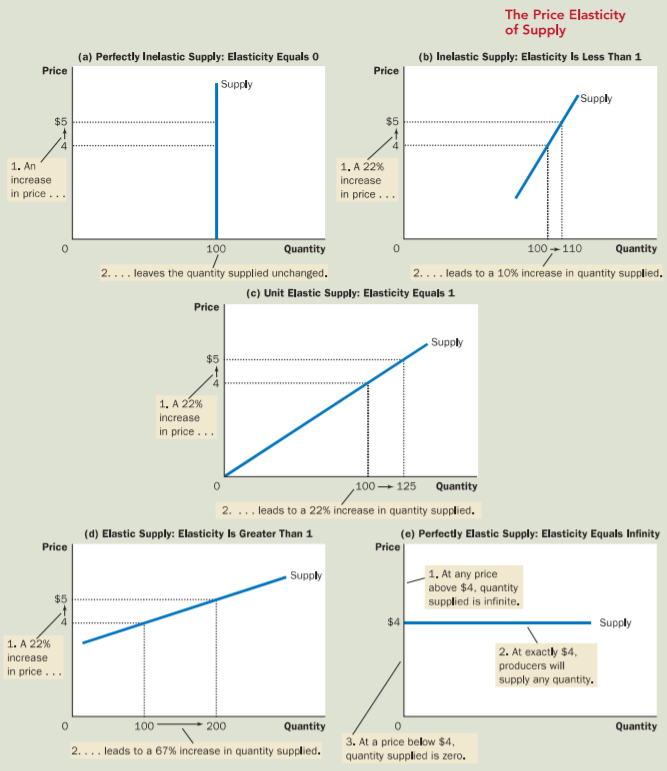
\includegraphics[width=14cm]{HS101 images/Diff. elasticity supply curves.png}
    \end{figure}
\e{itemize}

\phantomsection
\section*{\color{- }Supply, demand, and government policies}
\addcontentsline{toc}{section}{\large\color{- }Supply, demand, and government policies}
\b{itemize}
    \i \tb{price ceiling} - a legal maximum on the price at which a good can be sold
    \i \tb{price floor} - a legal minimum on the price at which a good can be sold
    \i If the price that balances supply and demand is below the ceiling, the price ceiling is {color{green}not binding}. Market forces naturally move the economy to the equilibrium, and the price ceiling has no effect on the price or the quantity sold. If the price is above the ceiling, the price ceiling is a {\color{green}binding} constraint on the market.
    \i When the government imposes a binding price ceiling on a competitive market, a shortage of the good arises, and sellers must ration the scarce goods among the large number of potential buyers
    \i If the equilibrium price is above the floor, the price floor is {color{green}not binding}. Market forces naturally move the economy to the equilibrium, and the price floor has no effect. If the price is below the floor, the price floor is a {\color{green}binding} constraint on the market.
    \i A binding price floor causes a surplus
    \i Minimum wage raises the incomes of those workers who have jobs, but it lowers the incomes of workers who cannot find jobs \i Rent control may keep rents low, but it also discourages landlords from maintaining their buildings and makes housing hard to find
\e{itemize}

\phantomsection
\section*{\color{- }Taxes}
\addcontentsline{toc}{section}{\large\color{- }Taxes}
\b{itemize}
    \i {\color{green}Taxes} are used to raise revenue for public projects, such as roads, schools, and national defense
    \i \tb{tax incidence} - the manner in which the burden of a tax is shared among participants in a market
    \begin{figure}[H]
    \centering
    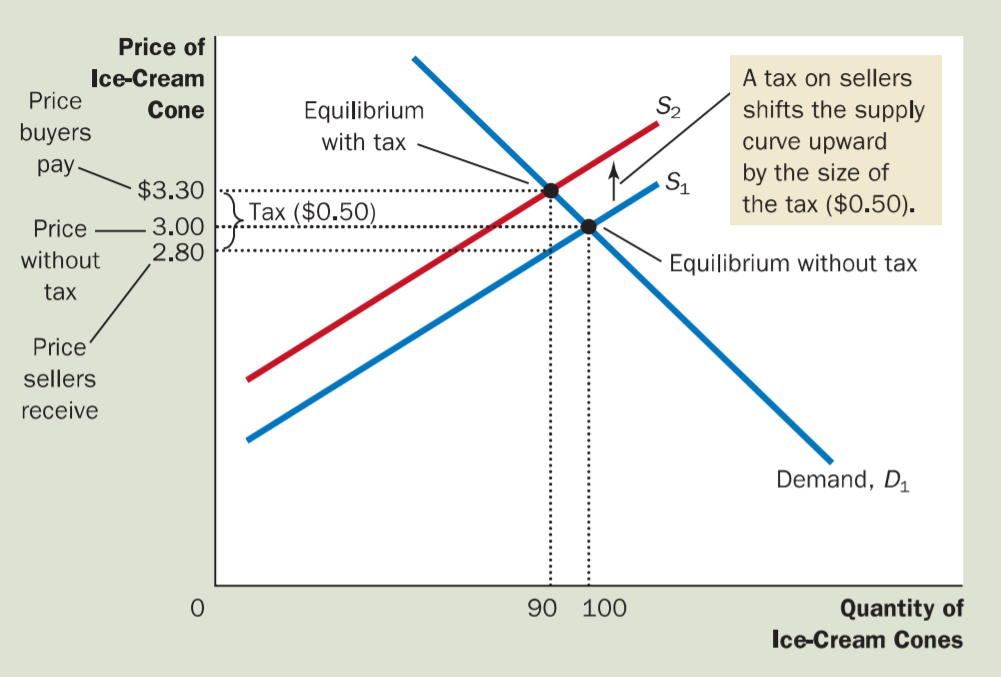
\includegraphics[width=9.5cm]{HS101 images/A tax on sellers.png}
    \caption{A tax on sellers}
    \end{figure}
    \begin{figure}[H]
    \centering
    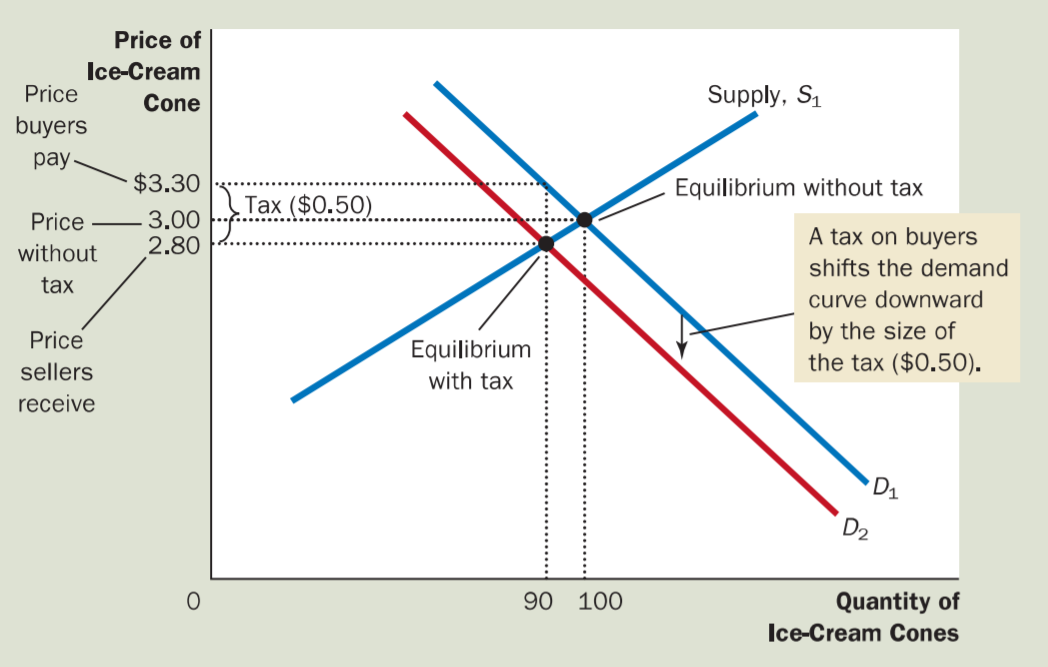
\includegraphics[width=9.5cm]{HS101 images/A tax on buyers.png}
    \caption{A tax on buyers}
    \end{figure}
    \i Taxes discourage market activity. When a good is taxed, the quantity of the good sold is smaller in the new equilibrium. Buyers ans sellers share the burden of taxes. In the new equilibrium, buyers pay more for the good, and sellers receive less. Therefore, taxes levied on buyers and taxes levied on sellers are equivalent
    \i \tb{payroll tax} - a tax on the wages that firms pay their workers
    \i A market with very elastic supply and relatively inelastic demand - buyers bear most of the burden of the tax
    \i A market with relatively inelastic supply and very elastic demand - sellers bear most of the burden of the tax
    \i A tax burden falls more heavily on the side of the market that is less elastic
    \i \tb{deadweight loss:} - the fall in total surplus that results from a market distortion, such as a tax
    \i The greater the elasticities of demand and supply the larger will be the decline in equilibrium quantity and, the greater the deadweight loss of a tax
    \i The economy is governed by two kinds of laws: the laws of supply and demand and the laws enacted by governments
\e{itemize}

\phantomsection
\section*{\color{- }Consumers, producers, and the efficiency of markets}
\addcontentsline{toc}{section}{\large\color{- }Consumers, producers, and the efficiency of markets}
\b{itemize}
    \i \tb{welfare economics} - the study of how the allocation of resources affects economic well-being
    \i \tb{willingness to pay} - the maximum amount that a buyer will pay for a good
    \i \tb{consumer surplus} - the amount a buyer is willing to pay for a good minus the amount the buyer actually pays for it
    \i The area below the demand curve and above the price measures the consumer surplus in a market
    \i \tb{cost} - the value of everything a seller must give up to produce a good
    \i \tb{producer surplus} - the amount a seller is paid for a good minus the seller's cost of providing it
    \i The area below the price and above the supply curve measures the producer surplus in a market
    \i \tb{total surplus} - it is the total value to the buyers of the goods, as measured by their willingness to pay, minus the total cost to sellers of providing those goods
    \i The total area between the supply and demand curves up to the point of equilibrium represent the total surplus in the market
    \i {\color{green}Free markets} allocate the supply of goods to the buyers who value them most highly, as measured by their willingness to pay. It allocates the demand for goods to the sellers who can produce them at the least cost. It produces the quantity of goods that maximizes the sum of consumer and producer surpluses.
\e{itemize}

\phantomsection
\section*{\color{- }The theory of consumer choice}
\addcontentsline{toc}{section}{\large\color{- }The theory of consumer choice}
\b{itemize}
    \i \tb{budget constraint} - the limit on the consumption bundles that a consumer can afford
    \i The slope of the budget constraint measures the rate at which the consumer can trade one good for the other
    \i \tb{indifference curve} - a curve that shows consumption bundles that give the consumer the same level of satisfaction
    \i \tb{marginal rate of substitution (MRS)} - the rate at which a consumer is willing to trade one good for another. This is the slope at any point on the indifference curve.
    \i Properties of indifference curves:
    \b{itemize}
        \item[$-$] Higher indifference curves are preferred to lower ones
        \item[$-$] Indifference curves are downward sloping
        \item[$-$] Indifference curves do not cross
        \item[$-$] Indifference curves are bowed inward
    \e{itemize}
    \i \tb{perfect substitutes} - two goods with straight-line indifference curves
    \i \tb{perfect complements} - two goods with right-angle indifference curves
    \i \tb{utility} - an abstract measure of the satisfaction or happiness that a consumer receives from a bundle of goods
    \i \tb{marginal utility} - with respect to a good, it is the increase in utility that the consumer gets from an additional unit of that good
    \i \tb{diminishing marginal utility} - the more of the good the consumer already has, the lower the marginal utility provided by an extra unit of that good
    \i The point at which the indifference curve and the budget constraint touch is called the {\color{green}optimum}
    \begin{figure}[H]
    \centering
    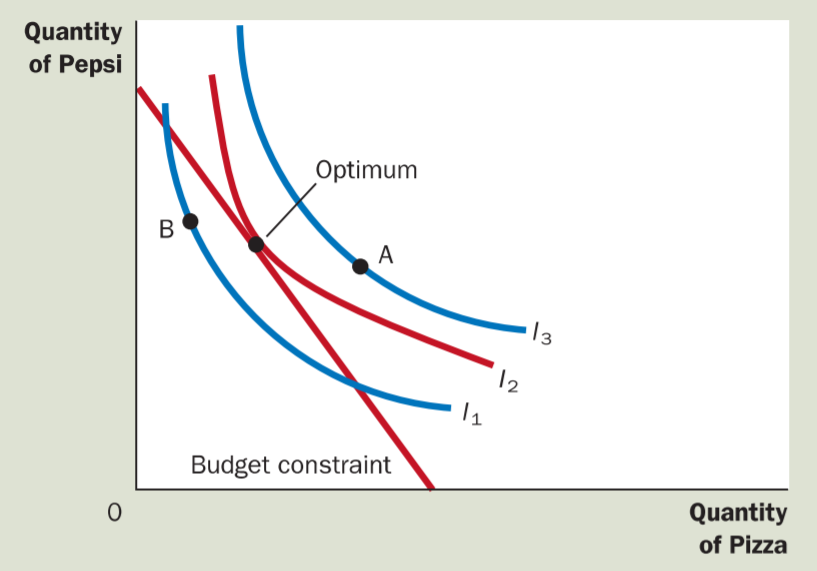
\includegraphics[width=9.5cm]{HS101 images/The consumer's optimum.png}
    \caption{The consumer's optimum}
    \end{figure}
    \i The consumer chooses consumption of the two goods so that the marginal rate of substitution equals the relative price
    \i \tb{income effect} - the change in consumption that results when a price change moves the consumer to a higher or lower indifference curve
    \i \tb{substitution effect} - the change in consumption that results when a price change moves the consumer along a given indifference curve to a point with a new marginal rate of substitution
    \i \tb{Giffen good} - a good for which an increase in the price raises the quantity demanded. They are inferior goods for which the income effect dominates the substitution effect. They have demand curves that slope upward.
\e{itemize}

\phantomsection
\section*{\color{- }The costs of production}
\addcontentsline{toc}{section}{\large\color{- }The costs of production}
\b{itemize}
    \i \tb{total revenue} - the amount a firm receives for the sale of its output
    \i \tb{total cost} - the market value of the inputs a firm uses in production
    \i \tb{total profit} - total revenue minus total cost
    \i \tb{explicit costs} - input costs that require an outlay of money by the firm
    \i \tb{implicit costs} - input costs that do not require an outlay of money by the firm
    \i \tb{economic profit} - total revenue minus total cost, including both explicit and implicit costs
    \i \tb{accounting profit} - total revenue minus total explicit cost
    \i \tb{production function} - the relationship between quantity of inputs used to make a good and the quantity of output of that good
    \i \tb{marginal product} - the increase in output that arises from an additional unit of input
    \i \tb{diminishing marginal product} - the property whereby the marginal product of an input declines as the quantity of the input increases
    \i \tb{fixed costs} - costs that do not vary with the quantity of output produced
    \i \tb{variable costs} - costs that vary with the quantity of output produced
    \i \tb{average total cost} - total cost divided by the quantity of output. The average total curve is U-shaped.
    \i \tb{average fixed cost} - fixed cost divided by the quantity of output
    \i \tb{average variable cost} - variable cost divided by the quantity of output
    \i \tb{marginal cost} - the increase in total cost that arises from an extra unit of production. It eventually rises with the quantity of output.
    \begin{figure}[H]
    \centering
    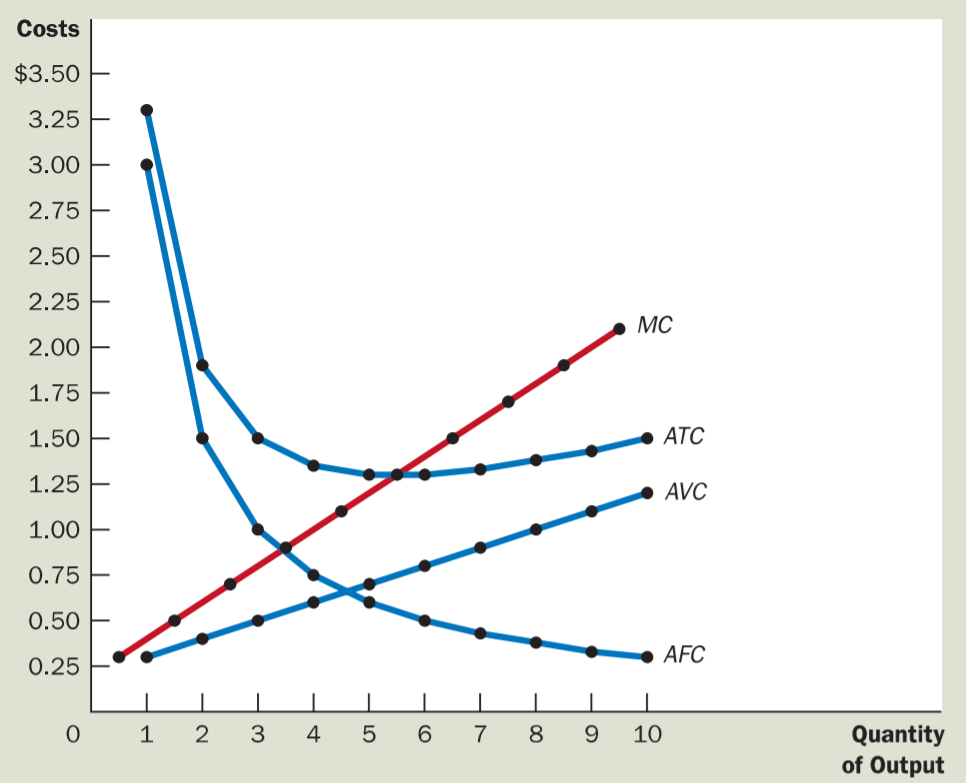
\includegraphics[width=9.5cm]{HS101 images/Cost curves.png}
    \caption{Cost curves}
    \end{figure}
    \i \tb{efficient scale} - the quantity of output that minimizes average total cost
    \i Whenever marginal cost is less than average total cost, average total cost is falling. Whenever marginal cost is greater than average total cost, average total cost is rising. The marginal cost curve crosses the average total cost curve at its minimum.
    \i \tb{economies of scale} - the property whereby in the long-run average total cost falls as the quantity of output increases
    \i \tb{diseconomies of scale} - the property whereby in the long-run average total cost rises as the quantity of output increases
    \i \tb{constant returns to scale} - the property whereby in the long-run average total cost stays the same as the quantity of output changes
    \begin{figure}[H]
    \centering
    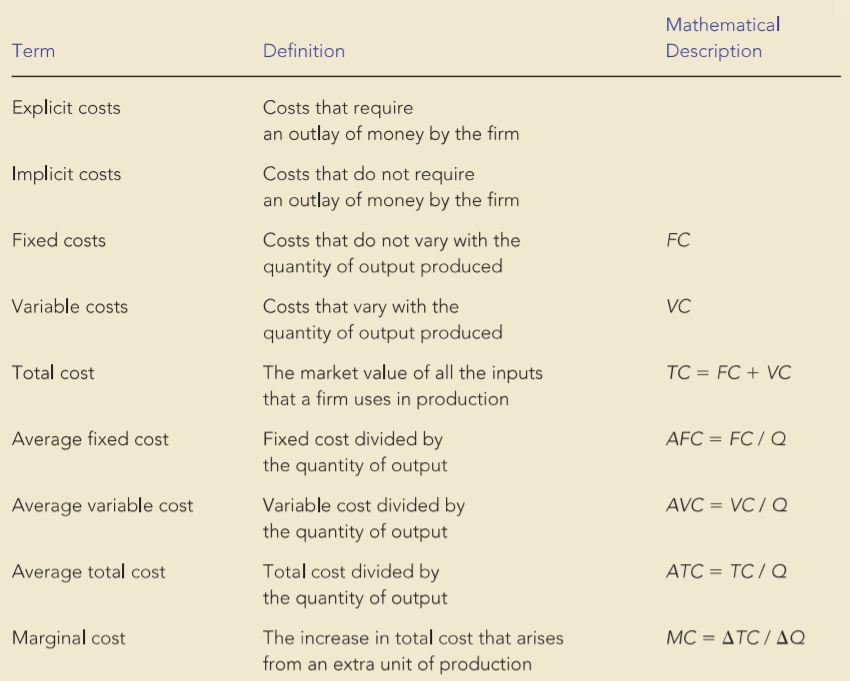
\includegraphics[width=9.5cm]{HS101 images/The many types of costs.png}
    \caption{The many types of costs}
    \end{figure}
\e{itemize}

\phantomsection
\section*{\color{- }Firms in competitive market}
\addcontentsline{toc}{section}{\large\color{- }Firms in competitive market}
\b{itemize}
    \i A firm is an organization that comes into being when a person or a group of people decides to produce a good or a service. A Firm can be organized in the form of {\color{green}sole proprietorship, partnership} or {\color{green}corporation.} Firms can be classified in terms of {\color{green}single} or {\color{green}multiple product firms}. They can also be classified in terms of {\color{green}domestic} and {\color{green}multinationals.}
    \i A competitive market is also called a {\color{green}perfectly competitive market}. It has three characteristics:
    \b{itemize}
        \item[$-$] There are many buyers and many sellers in the market
        \item[$-$] The goods offered by the various sellers are largely the same
        \item[$-$] Firms can freely enter or exit the market
    \e{itemize}
    \i Buyers and sellers in competitive markets must accept the price the market determines and, therefore, are said to be {\color{green}price takers}
    \i \tb{average revenue} - total revenue divided by the quantity sold. For all firms, average revenue equals the price of the good.
    \i \tb{marginal revenue} - the change in total revenue from an additional unit sold. For competitive firms, marginal revenue equals the price of the good.
    \i \tb{marginal revenue product (MRP)} - MRP of the variable input equals the marginal product (MP) of the variable input times the marginal revenue (MR) from the sale of the extra output produced
    \i \tb{marginal resource cost (MRC)} - MRC of a variable input is equal to the increase in total costs resulting from hiring an additional unit of the variable input
    \i As long as MRP exceeds MRC, it pays for the firm to expand the use of the variable input used because by doing so, it adds more to its total revenue than to its total cost (so that the firms total profits rise)
    \i Three general rules for profit maximization:
    \b{itemize}
        \item[$-$] If marginal revenue is greater than marginal cost, the firm should increase its output 
        \item[$-$] If marginal cost is greater than marginal revenue, the firm should decrease its output
        \item[$-$] At the profit-maximizing level of output, marginal revenue and marginal cost are exactly equal
    \e{itemize}
    \begin{figure}[H]
    \centering
    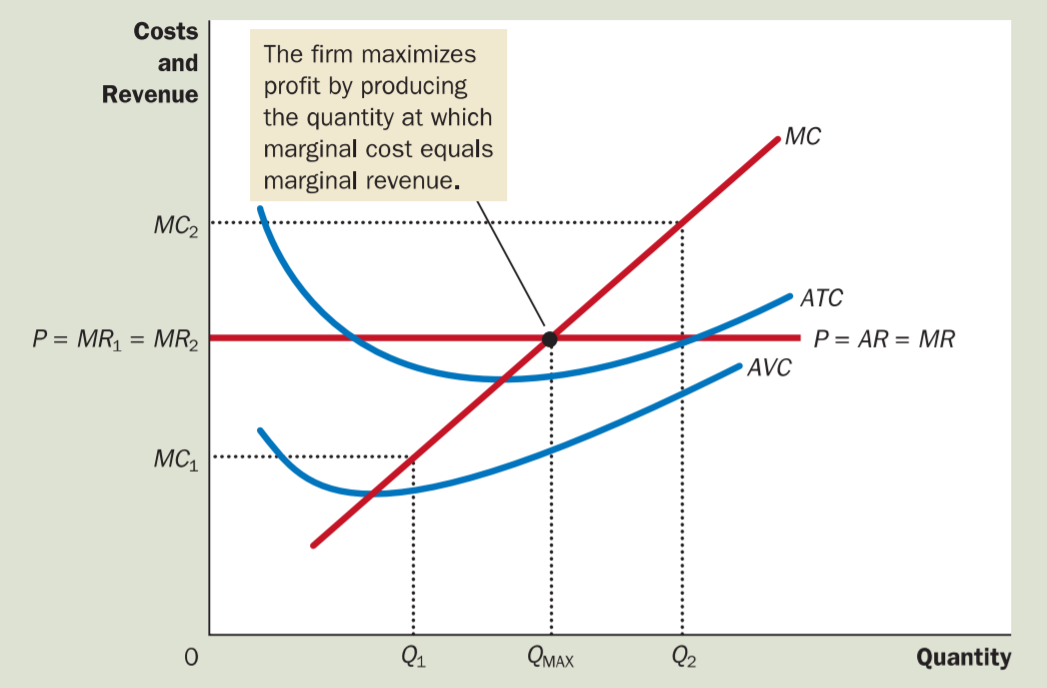
\includegraphics[width=9.5cm]{HS101 images/Profit maximization for a competitive firm.png}
    \caption{Profit maximization for a competitive firm}
    \end{figure}
    \i A {\color{green}shutdown} refers to a short-run decision not to produce anything during a specific period of time because of current market conditions
    \i {\color{green}Exit} refers to a long-run decision to leave the market
    \i The reason firms shut down is because the revenue that it would get from producing is less than its variable cost
    \i The competitive firm's short-run supply curve is the portion of its marginal-cost curve that lies above average variable cost
    \i \tb{sunk cost} - a cost that has already been committed and cannot be recovered
    \i The reason firms exit is because the revenue that it would get from producing is less than its total cost
    \i The competitive firm's long-run supply curve is the portion of its marginal-cost curve that lies above average total cost
    \i Profit can be found by the following equation:
    \begin{figure}[H]
    \centering
    
\includegraphics[width=4cm]{HS101 images/Profit equation.png}
    \end{figure}
    where $P$ is the price (average revenue) and $Q$ is the quantity
    \i Reasons of a long-run supply curve sloping upwards:
    \b{itemize}
        \item[$-$] Some resources used in production may be available only in limited quantities
        \item[$-$]Firms may have different costs
    \e{itemize}
    \i \tb{law of equi-marginal utility} - at the point of equilibrium, the consumer’s substitution ratio is just equal to the slope of the budget line
    \i \tb{Pareto efficiency} (also known as just efficiency) occurs when no possible reorganisation of production or distribution can make anyone better off without making someone else worse off
\e{itemize}

\phantomsection
\section*{\color{- }The data of macroeconomics}
\addcontentsline{toc}{section}{\large\color{- }The data of macroeconomics}
\b{itemize}
    \i \tb{gross domestic product (GDP)} - is the market value of all final goods and services produced within a country in a given period of time. It measures two things at once: the total income of everyone in the economy and the total expenditure on the economy’s output of goods and services.
    \i For an economy as a whole, income must equal expenditure
    \i GDP excludes items produced and sold illicitly, such as illegal drugs. It also excludes most items that are produced and consumed at home and, therefore, never enter the marketplace. It includes only the value of final goods. The reason is that the value of intermediate goods is already included in the prices of the final goods.
    \i GDP includes goods and services currently produced. It does not include transactions involving items produced in the past. It measures the value of production within the geographic confines of a country.
    \i \tb{gross national product (GNP)} - is the total income earned by a nation’s permanent residents (called nationals). It differs from GDP by including income that our citizens earn abroad and excluding income that foreigners earn here.  For most countries, domestic residents are responsible for most domestic production, so GDP and GNP are quite close.
    \i \tb{net domestic product} - is obtained by subtracting depreciation from GDP
    \i \tb{net national product (NNP)} - is the total income of a nation’s residents (GNP) minus losses from depreciation. Depreciation is the wear and tear on the economy’s stock of equipment and structures. 
    \i \tb{national income} - is the total income earned by a nation’s residents in the production of goods and services. It differs from net national product by excluding indirect business taxes (such as sales taxes) and including business subsidies. NNP and national income also differ because of a “statistical discrepancy” that arises from problems in data collection.
    \i \tb{personal income} - is the income that households and noncorporate businesses receive. Unlike national income, it excludes retained earnings, which is income that corporations have earned but have not paid out to their owners. It also subtracts corporate income taxes and contributions for social insurance (mostly Social Security taxes). In addition, personal income includes the interest income that households receive from their holdings of government debt and the income that households receive from government transfer programs, such as welfare and Social Security.
    \i \tb{disposable personal income} - is the income that households and noncorporate businesses have left after satisfying all their obligations to the government. It equals personal income minus personal taxes and certain nontax payments (such as traffic tickets).
    \i When the government reports quarterly GDP, it presents the data after they have been modified by a statistical procedure called {\color{green}seasonal adjustment.} This is the process by which government statisticians adjust the quarterly data to take out the seasonal cycle.
    \i GDP (which we denote as $Y$) is divided into four components: consumption ($C$), investment ($I$), government purchases ($G$), and net exports ($NX$). Now, its equation is:
    $$Y=C+I+G+NX$$
    \i \tb{consumption} - spending by households on goods and services, with the exception of purchases of new housing
    \i \tb{investment} - spending on capital equipment, inventories, and structures, including household purchases of new housing
    \i \tb{government purchases} - spending on goods and services by local, state, and federal governments
    \i \tb{net exports} - spending on domestically produced goods by foreigners (exports) minus spending on foreign goods by domestic residents (imports)
    \i A {\color{green}transfer payment} is not made in exchange for a currently produced good or service. From a macroeconomic standpoint, transfer payments are like a tax rebate. Like taxes, transfer payments alter household income, but they do not reflect the economy’s production. Because GDP is intended to measure income from (and expenditure on) the production of goods and services, transfer payments are not counted as part of government purchases.
    \i \tb{nominal GDP} - the production of goods and services valued at current prices
    \i \tb{real GDP} - the production of goods and services valued at constant prices. Real GDP is calculated by first choosing one year as a {\color{green}base year.}
    \i \tb{GDP deflator/price of GDP} - a measure of the price level calculated as the ratio of nominal GDP to real GDP times 100. It's equation is:
    $$ \text{GDP deflator} = \frac{\text{Nominal GDP}}{\text{Real GDP}}\times 100 $$
    \i \tb{recession} - is a period of significant decline in total output, income, and employment, usually lasting more than a few months and marked by widespread contractions in many sectors of the economy. A good rule of thumb to spot a recession is two consecutive quarters of falling real GDP. A severe and protracted downturn is called a {\color{green}depression.}
    \i \tb{business cycle} - is the short-term fluctuations in output, employment, financial conditions, and prices
    \i \tb{economic growth} - is the long-term trends in output and living standards
    \i \tb{stagflation} - period of slow growth and rising prices
    \i The key factors in long-term economic growth include reliance on well-regulated private markets for most economic activity, stable macroeconomic policy, high rates of saving and investment, openness to international trade, and accountable and noncorrupt governing institutions
    \i \tb{Keynesian economics} - {\color{green}John Maynard Keynes} in his 1936 book, {\color{green}The General Theory of Employment, Interest, and Money}, made a twofold argument: First, he argued that it is possible for high unemployment and underutilized capacity to persist in market economies. In addition, he argued that government fiscal and monetary policies can affect output and thereby reduce unemployment and shorten economic downturns.
    \i Objectives and instruments of macroeconomic policies:
    \b{itemize}
        \item[$-$] Objectives:
        \b{itemize}
            \item[$\diamond$] \tb{output:} high level and rapid growth of output
            \item[$\diamond$] \tb{employment:} high level of employment with low involuntary unemployment
            \item[$\diamond$] \tb{stable prices}
        \e{itemize}
        \item[$-$] Instruments:
        \b{itemize}
            \item[$\diamond$] \tb{monetary policy:} buying and selling bonds, regulating financial institutions
            \item[$\diamond$] \tb{fiscal policy:} government expenditures, taxation
        \e{itemize}
    \e{itemize}
    \i \tb{potential GDP} -  represents the maximum sustainable level of output that the economy can produce. When an economy is operating at its potential, there are high levels of utilization of the labor force and the capital stock. When output rises above potential output, price inflation tends to rise, while a below-potential level of output leads to high unemployment. Potential output is determined by the economy’s productive capacity, which depends upon the inputs available (capital, labor, land, etc.) and the economy’s technological efficiency. Potential GDP tends to grow steadily because inputs like labor and capital and the level of technology change quite slowly over time. By contrast, actual GDP is subject to large business-cycle swings if spending patterns change sharply.
    \i \tb{price indexes} - are measures of the overall price level constructed by government statisticians to track prices. It is a weighted average of the price of a basket of goods and services. In constructing price indexes, economists weight individual prices by the economic importance of each good. The most important price indexes are the consumer price index, the GDP price index, and the producer price index
    \i \tb{consumer price index (CPI)} - measures the trend in the average price of goods and services bought by consumers. The overall price level is generally denoted by the letter P.
    \i \tb{rate of inflation:}
    $$\text{Rate of inflation in year }t=\frac{P_t-P_{t-1}}{P_{t-1}}\times 100 $$
    \i A {\color{green}deflation} occurs when prices decline (which means that the rate of inflation is negative). At the other extreme is a {\color{green}hyperinflation}, a rise in the price level of a thousand or a million percent a year.
    \i A {\color{green}policy instrument} is an economic variable under the control of government that can affect one or more of the macroeconomic goals. By changing monetary, fiscal, and other policies, governments can avoid the worst excesses of the business cycle or increase the growth rate of potential output.
    \i \tb{fiscal policy} -  denotes the use of taxes and government expenditures. Government expenditures come in two distinct forms. First there are {\color{green}government purchases.} These comprise spending on goods and services — purchases of tanks, construction of roads, salaries for judges, and so forth. In addition, there are {\color{green}government transfer payments,} which increase the incomes of targeted groups such as the elderly or the unemployed. Government spending determines the relative size of the public and private sectors, that is, how much of our GDP is consumed collectively rather than privately. From a macroeconomic perspective, government expenditures also affect the overall level of spending in the economy and thereby influence the level of GDP. 
    \i \tb{monetary policy} - is the second major instrument of macroeconomic policy, which the government conducts through managing the nation’s money, credit, and banking system. It is conducted by the central bank, determines short-run interest rates. It thereby affects credit conditions, including asset prices such as stock and bond prices and exchange rates. Changes in interest rates, along with other financial conditions, affect spending in sectors such as business investment, housing, and foreign trade. Monetary policy has an important effect on both actual GDP and potential GDP. 
    \i \tb{globalization} - is the phenomenon by which nations participate in the world economy and are linked together through trade and finance
    \i \tb{balance on current account} - represents the numerical difference between the value of exports and the value of imports, along with some other adjustments. When exports exceed imports, the difference is a surplus, while a negative balance is a deficit.
    \i  \tb{aggregate supply} refers to the total quantity of goods and services that the nation’s businesses willingly produce and sell in a given period. Aggregate supply (often written AS) depends upon the price level, the productive capacity of the economy, and the level of costs.
    \i \tb{aggregate demand} refers to the total amount that different sectors in the economy willingly spend in a given period. Aggregate demand (often written AD) equals total spending on goods and services. It depends on the level of prices, as well as on monetary policy, fiscal policy, and other factors.
    \begin{figure}[H]
    \centering
    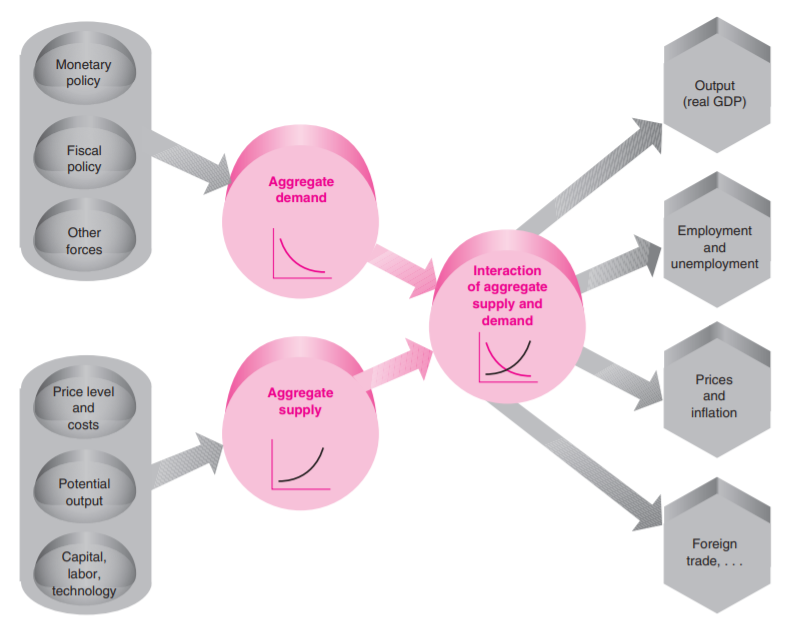
\includegraphics[width=14cm]{HS101 images/AS and AD determine the major macroeconomic variables.png}
    \caption{AS and AD determine the major macroeconomic variables}
    \end{figure}
    \i The downward-sloping curve from the figure above is the {\color{green}aggregate demand schedule,} or {\color{green}AD curve.} It represents what everyone in the economy —consumers, businesses, foreigners, and governments would buy at different aggregate price levels (with other factors affecting aggregate demand held constant).
    \i The upward-sloping curve is the {\color{green}aggregate supply schedule,} or {\color{green}AS curve.} This curve represents the quantity of goods and services that businesses are willing to produce and sell at each price level (with other determinants of aggregate supply held constant).
    \i A {\color{green}macroeconomic equilibrium} is a combination of overall price and quantity at which all buyers and sellers are satisfied with their overall purchases, sales, and prices
    \i An {\color{green}account} for a firm or nation is a numerical record of all flows (outputs, costs, etc.)
    \i Value added is the difference between a firm’s sales and its purchases of materials and services from other firms
    \i When relative prices of different goods are changing very rapidly, using prices of a fixed year will give a misleading estimate of real GDP growth. To correct for this bias, statisticians use a procedure known as {\color{green}chain weighting.} Instead of the relative weights on each good being kept fixed (say, by the use of weights for a given year, like 1990), the weights of the different goods and services change each year to reflect the changes in spending patterns in the economy.
    \i Economists define “investment” (or sometimes {\color{green}real investment}) as production of durable capital goods. In common usage, “investment” often denotes using money to buy General Motors stock or to open a savings account. For clarity, economists call this {\color{green}financial investment.} Try not to confuse these two different uses of the word “investment.” If we take some money and buy some stocks, this is not what macroeconomists call investment. We have simply exchanged one financial asset for another. Investment takes place when a durable capital good is produced.
    \i \tb{gross investment} - includes all investment goods produced. It is not adjusted for depreciation, which measures the amount of capital that has been used up in a year.
    \i \tb{net investment} - is gross investment minus depreciation
    \begin{figure}[H]
    \centering
    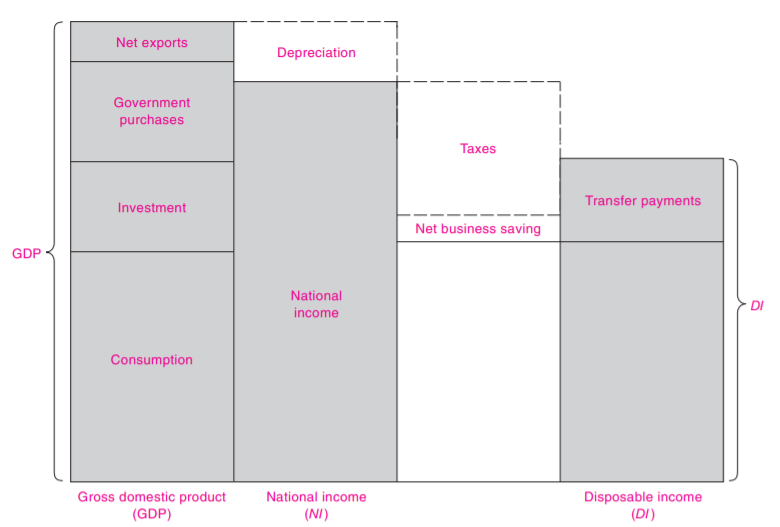
\includegraphics[width=14cm]{HS101 images/From GDP to National Income to Disposable Income.png}
    \caption{From GDP to National Income to Disposable Income}
    \end{figure}
    \i National saving equals national investment by definition. The components of investment are private domestic investment and foreign investment (or net exports). The sources of saving are private saving (by households and businesses) and government saving (the government budget surplus). Private investment plus net exports equals private saving plus the budget surplus. These identities must hold always, whatever the state of the business cycle.
    \i  \tb{underground economy} covers a wide variety of market activities that are not reported to the government. These include activities like gambling, prostitution, drug dealing, work done by illegal immigrants, bartering of services, and smuggling.
    \i \tb{Okun's law} - is an empirically observed relationship between unemployment and losses in a country's production. It is named after Arthur Melvin Okun, who first proposed the relationship in 1962. The "gap version" states that for every 1$\%$ increase in the unemployment rate, a country's GDP will be roughly an additional 2$\%$ lower than its potential GDP. 
\e{itemize}

\e{document} 

